\begin{frame}{}
    \LARGE VAE: \textbf{Evidence Lower Bound (ELBO)}
\end{frame}

\begin{frame}[allowframebreaks]{Evidence Lower Bound (ELBO)}
\textbf{What is ELBO?}:
\begin{itemize}
    \item Allows us to optimize the model.
    \item It provides a lower bound on the log-likelihood of the data, which we aim to maximize during training.
    \item The ELBO consists of two main components:
    \begin{itemize}
        \item \textbf{Reconstruction term}: Measures how well the model can reconstruct the input data from the latent representation.
        \item \textbf{Regularization term}: Encourages the learned latent distribution to be close to a prior distribution (usually Gaussian).
    \end{itemize}
    \framebreak
    \item Mathematically, the ELBO can be expressed as:
    \[
    \mathcal{L}(\theta, \phi; x) = \mathbb{E}_{q_\phi(z|x)}[\log p_\theta(x|z)] - D_{KL}(q_\phi(z|x) \| p(z))
    \]
    where:
    \begin{itemize}
        \item \( q_\phi(z|x) \) is the approximate posterior distribution (encoder).
        \item \( p_\theta(x|z) \) is the likelihood of the data given the latent variable (decoder).
        \item \( D_{KL} \) is the Kullback-Leibler divergence between the approximate posterior and the prior distribution \( p(z) \).
    \end{itemize}
    \item The goal is to maximize the ELBO with respect to the model parameters \( \theta \) and \( \phi \).
    \item By maximizing the ELBO, we ensure that the model learns a meaningful latent representation while also being able to generate new samples.
\end{itemize}

\framebreak

Looking at Lower bound $L$
\begin{equation*}
    \begin{split}
        L & = \sum_z q(z) log \frac{p(x,z)}{q(z)}\\
        & = \sum_z q(z) log \frac{p(x|z)p(z)}{q(z)}\\
        & = \sum_z q(z) \left [log \, p(x|z) + log \frac{p(z)}{q(z)} \right ]\\
        & = \underbrace{\sum_z q(z) log \, p(x|z)}_{\text {Expectation} \, E_{q(z)}(log \, p(x|z))} + \underbrace{\sum_z q(z) log \frac{p(z)}{q(z)}}_{-KL(q(z)||p(z)} \\
    \end{split}
\end{equation*}
So,
$$L = E_{q(z)}(log \, p(x|z)) - KL(q(z)||p(z))$$

\framebreak
\begin{itemize}
    \item $E_{q(z)}(log \, p(x|z))$ is conceptually reconstruction
    \item We can assume $z$ to be Standard Normal Distribution
\end{itemize}
\vspace{1em}
\begin{figure}
    \centering
    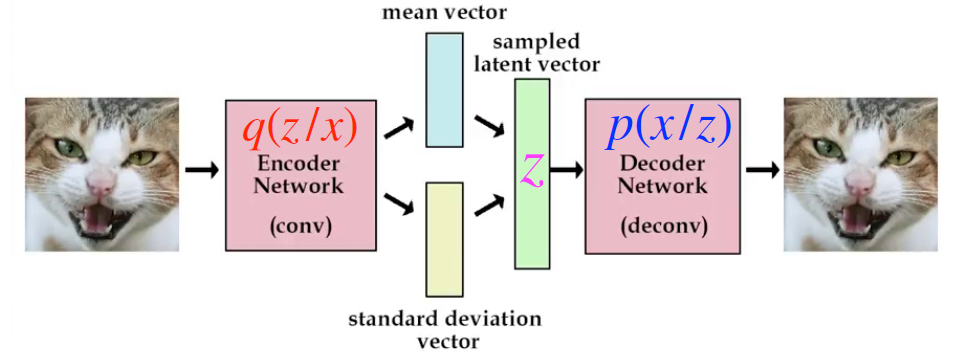
\includegraphics[height=0.5\textheight, width=\textwidth, keepaspectratio]{images/vae/architecture.png}
    \caption*{Variational Autoencoder Architecture}
\end{figure}

\framebreak
\begin{figure}
    \centering
    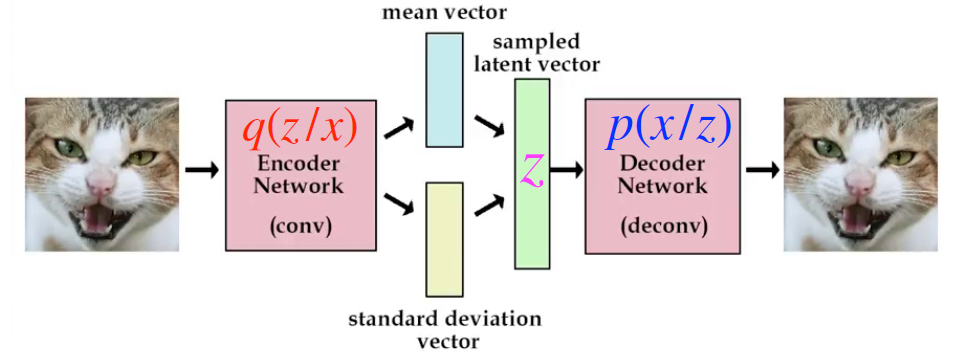
\includegraphics[height=0.3\textheight, width=\textwidth, keepaspectratio]{images/vae/architecture.png}
\end{figure}
$$p(x|\hat{x}) = e^{-|x-\hat{x}|^2}$$
$$log \, e^{-|x-\hat{x}|^2} = -|x-\hat{x}|^2$$
$$L = E_{q(z)}(-|x-\hat{x}|^2) - KL(q(z)||p(z))$$
$$\min |x-\hat{x}| + KL(q(z|x)||\mathcal{N}(0,1))$$
$$\min |x-\hat{x}| - 0.5 * (1 + log \, \sigma^2 - \sigma^2 - \mu^2)$$

For full derivation of KL Loss, read \href{https://deepai.org/publication/tutorial-deriving-the-standard-variational-autoencoder-vae-loss-function}{here}
\end{frame}